\chapter{Theoretical Background}
\label{chap:terms}
 \section {Forced Alignment and Timing} 
One of the central algorithm  of the modern ASRs is  a token passing
algorithm. Recognition is the process of producing hypotheses, that fit best
with the audio input. During decoding these hypotheses are
saved as a list of tokens, which contains information about alignment, states
and transitions. \parencite {Young89Token}.
\begin{figure}[htbp]
  \centering
   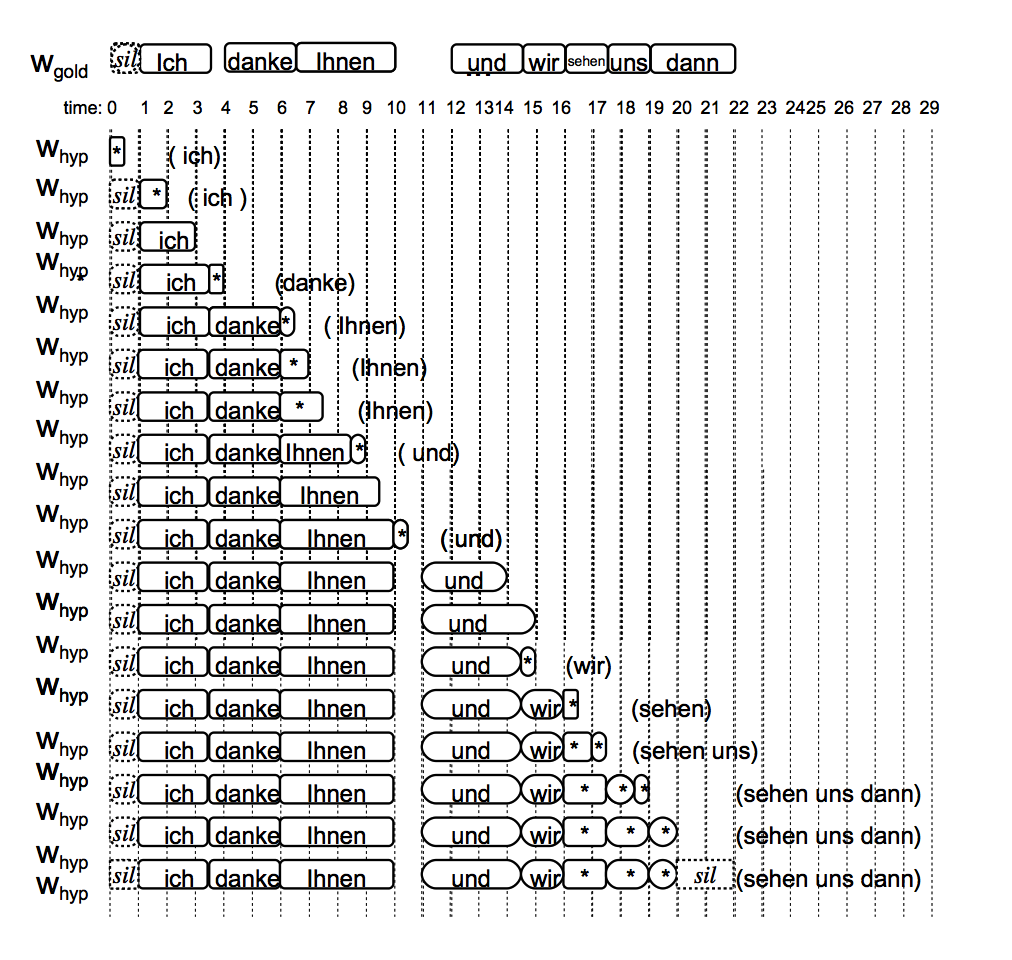
\includegraphics[width=1\textwidth]{images/sphinxfa_output.png}
  \caption{Incremental output of Sphinx ASR, running in the forced alignment
  mode.}
  \label{fig:sphinxfa}
\end{figure}

Generally, \textit {forced alignment} is the process of finding the
correspondence between a piece of text and audio speech segments. In the case,
when the transcription is known \textit {forced alignment} consists only in
determining where in time these particular words occur in the speech segment. 
For example, if we take transcription \textit {ich danke Ihnen und wir sehen uns
dann} and run Sphinx ASR in the forced alignment mode with the corresponding
audio input than we get the following incremental output (see \ref
{fig:sphinxfa}).
By giving the transcription to the recogniser we narrow its search space for hypotheses to
one particular path. Even if the recognizer receives some text, that differs
from the \textit {gold standard} text, pronounced in our audio, it will still try to
align it to the audio as good as possible. 
\begin{figure}[htbp]  
  \centering
   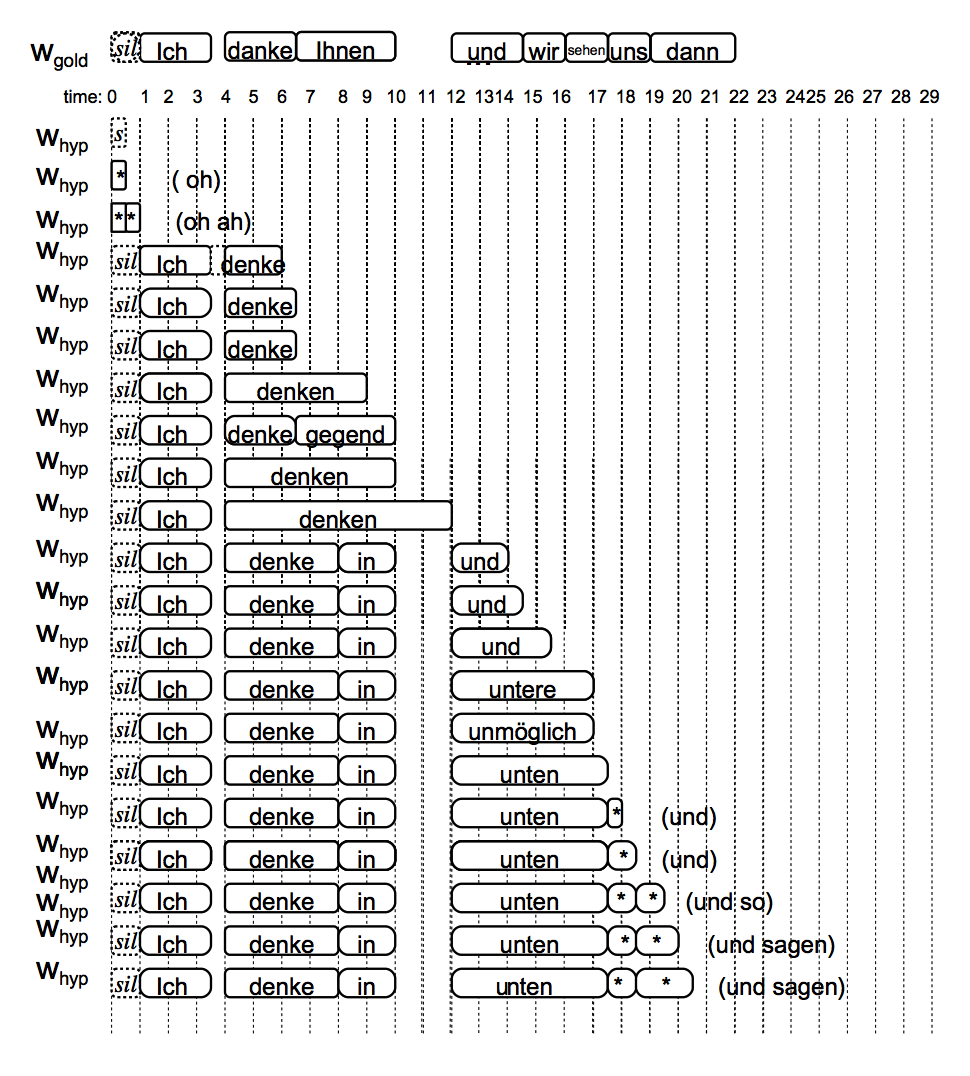
\includegraphics[width=1\textwidth]{images/sphinx_output.png}
  \caption{Incremental output of Sphinx ASR, running in the normal recognition
  mode.}
  \label{fig:sphinx}
\end{figure}
By contrast, during normal recognition we are dealing with numerous paths  and
possible states in the search graph. During decoding alignment
is computed synchronously together with search states. Final path can differ
from \textit {gold standard} transcription, depending on the recognition
quality.
The more further recognizer in their hypotheses from the original transcription the
worse is the recognition quality. Comparison between two sphinx outputs
(see pictures \ref {fig:sphinxfa} and \ref {fig:sphinx}) makes it obvious that
alignment quality depends on the recognition quality.

\textit {Forced alignment} is of great importance in fast-moving environments,
where additional non-verbal information pieces, for example gestures, are used. 
Without timing information in such kind of applications it not always possible to
analyse correctly which object is referenced 
\parencite {Baumann2016}.  In contrast to Sphinx, online Google, being a black
box, does not output alignment timing, which makes it impossible to use this 
recognizer for applications, using non-verbal information and context-dependent
object referencing. 

\section {Alignment Quality Metrics}
Alignment quality metrics describe how good is the timing of the output,
produced by the recognizer, compared with the \textit {gold standard}. The main
metrics that can be used for this purpose are: \textit {mean error}, \textit {standard deviation} and 
and \textit {root mean squared error}. In this paper we
differentiate between incremental and non-incremental approach to the
calculation of the errors.  For non-incremental approach only the
final timing result of the recognizer are compared with the \textit {gold
standard}. By contrast, incremental approach requires to compare incremental
timing results with \textit {gold standards}.  How exactly the errors are
computed is explained in details in the subsections below. 
\subsection {Mean Error} \textit {Mean error}  $\mu$ 
describes the average of absolute errors. Reformulated in accordance with
the alignment problem of a recognizer  \textit {mean error}   can be expressed
mathematically as follows:
\begin{center} 
\begin{equation} \mu=\frac{\sum_{i=0}^N
|t_{i_{start}(rec)}-t_{i_{start}(gold)}|+|t_{i_{end}(rec)}-t_{i_{end}(gold)}|}{N}
\label{eq:mean}
\end{equation}
\end{center} In the formula  \ref {eq:mean}, shown above, 
$t_{i_{start}(rec)}$ and $t_{i_{end}(rec)}$ equals the start and the end of a
matched or substituted word in the recognizer output,
$t_{i_{start}(gold)}$ and $t_{i_{end}(gold)}$ equals the start and the end of
a corresponding word in the gold standard and $N$ is the total number of matches
and substitutions or only matches.

In the case of the forced alignment of a phrase, that is equal with the
transcription, the total number of matches and substitutions is equals the
number of words (compare \ref{fig:sphinx}). When ASR runs in the normal
recognition mode the number of matches and substitutions can differ from the number of words as we are possibly  dealing with some deletions or insertions. Matches and
substitutions are relatively easily obtained from the 
Levenshtein distance matrix, containing substitutions, matches, deletions and
insertions of characters, occurring in two strings \parencite {levenshtein1966}.  

For the above example (figure \ref{fig:sphinx}) the mean  error, related to
the final result \textit {Ich danke ihnen und wir sehen uns dann}, is computed
as follows:
\begin{equation} \mu=\frac{(0+100+50+150+0+0+0+200)}{8} \approx 50 ms
\label{eq:mean_comp}
\end{equation}

For incremental approach it is necessary first to calculate the \textit {
 mean error} of the incremental results for every word, belonging to the final match or
substitution. In addition, we have to consider only incremental results with
changing timings. As soon as the result is stable it is not any more significant
for the analysis of timing incrementality. The reason is that the words in the
beginning of the utterance appear ofter in the hypotheses and will minimize their error with
every new hypotheses, if the mean error is computed over all of them.  

In the example above (figure \ref{fig:sphinx}) the word \textit  {ich} 
appears 18 times in the output, but only first 4 outputs are relevant for incremental timing
analyses.  Starting from the 5-th incremental result the timing for the \textit
{ich} does not change any more.  The mean error of the word \textit {ich} for
the first 4 incremental results equals $\frac {400+200+50+0}{4}\approx 163 ms$, whereas for 18 incremental results 
it equals only $\frac {400+200+50+0*15}{18}=\approx 36 ms$. 

The \textit {mean error} for all words in incremental case in the above example
(figure \ref{fig:sphinx}) is the following:

\begin{equation} \mu=\frac{(163 +200 +240 +233 +225+67+83+250)}{8} \approx 183 ms
\label{eq:mean_comp_inc}
\end{equation}

\subsection {Standard Deviation}
\textit {Standard deviation} is the square root of its variance
:\begin{equation} \sigma=\sqrt {Var}
\end{equation}
\textit {Variance} $Var(X)$ in its turn is the average of the squared
differences from the \textit {mean}:
\begin{equation} Var(X)=\frac{\sum_{i=0}^N (t_i(rec)-\mu)2}{N}
\end{equation}
In the above formula $t_i(rec)$ is the actual recognizer timing and $N$ is again
is the number of matches and substitutions.  Standard deviation in the Sphinx
example (figure \ref{fig:sphinx}) with non-incremental approach is calculated as
shown below:
\begin{equation} \sigma=\sqrt {\frac
{2500+2500+0+10000+2500+2500+2500+22500}{8}}\approx 75 ms
\end{equation}

For incremental case $\sigma$ is first computed for every word in the utterance
as the average of the squared differences of all relevant incremental results from
the mean (equation \ref{eq:mean_comp_inc}). For the word \textit {ich} in the
above example (figure \ref{fig:sphinx}) it equals:
\begin{equation} \sigma=\sqrt {\frac
{(400-183)^2+(200-183)^2+(50-183)^2+(0-183)^2}{4}}\approx 157 ms
\end{equation}

Finally, the $\sigma$ for all words is computed as an average of the sigmas of
all the words in the utterance:
\begin{equation} \sigma_{incr}=\frac
{(157+101+ 201+138+342+ 84 +79 +168 )}{8}\approx 159
ms
\end{equation}


\subsection {Root Mean Squared Error}
\textit {Root mean squared error} (RMSE) is the square root of  \textit {mean
error}  and \textit {standard deviation} \begin{equation} RMSE=\sqrt
{\mu^2+\sigma^2}. 
\end{equation}
For the Sphinx example above  (figure \ref{fig:sphinx}) in  non-incremental case
it equals:
\begin{equation} RMSE=\sqrt
{50^2+75^2} \approx 90 ms. 
\end{equation}

In the incremental case the result equals:
\begin{equation} RMSE=\sqrt
{183^2+159^2} \approx 242 ms. 
\end{equation}



\section {Timeliness in Speech Recognition} 
\textit {Timeliness} is the second term that is used to characterize word
occurrences during recognition in relation to the time axis. 
To describe the term \textit {timeliness} the following evaluation metrics are
used:
\begin{itemize}
  \item First Occurrence (FO) - is the time between the (true) beginning of a
  word and the first time it occurs in the output (regardless if it is afterwards changed).
\item Final Decision (FD) - is the time between the (true) end of a word and the
time when the recognizer decides on the word, without later revising it anymore.
\end{itemize}

\textit {Timeliness} is only measured for the words that are correctly
recognized or at least appear in the final output of the recognizer \parencite
{Baumann2016}.

\textit {Timeliness} characterizes, how fast is the recognizer in its
hypotheses. In the above depicted output of Sphinx ASR (see figures \ref
{fig:sphinxfa} and \ref {fig:sphinx}) FO as well as FD of the word \textit {ich}  in the first
case (forced alignment mode) takes plays a half of the slot earlier than in the second case (normal
recognition) and before the word \textit {ich} ends in the audio. 

Metrics that are used in this thesis for the timeliness quality evaluation are:
mean, standard deviation and median. For the above example (see figure \ref
{fig:sphinxfa} ) mean is computed as shown below:
\begin{equation} \mu (FO)=\frac{((-50) +0 +(-50)+(-300)+ 50+50+0+0)}{8} \approx
-37,5 ms
\label{eq:mean_comp_inc}
\end{equation}


For standard deviation we have:
\begin{equation}
\begin{aligned}
\sigma=
\sqrt {\frac{156,25 +1406,25 +156,25 +68906,25+}{8}}\ldots\\
\ldots\sqrt {\frac{+156,25+156,25+1406,25+1406,25}{8}}\approx 34ms\\
\end{aligned}
\end{equation}
Median, which is the ``middle'' value of the data set,  equals 0. For FD the quality metrics are calculated analogue. 
 





 

 